\section{Phase 4: Load Balancing with Fault Tolerance}\label{sec:phase4}

\subsection{Failure Experiment}
The load generator sends requests through the LB at \textbf{[R]}\,req/s for 60\,s.
After 20\,s we stop \texttt{server2} with \texttt{docker stop} and check the containers
with \texttt{docker ps -a}; after 40\,s we start it again with \texttt{docker start}. From the per-request results we plot how many requests each
server answered per second, and how many failed (Fig.~\ref{fig:timeline}). We ran
this for both algorithms, first with the Phase~3 LB (health checks switched off)
and then with the Phase~4 LB.

\subsection{Failure Without Fault Tolerance}
% TODO check in your Phase 3 runs which errors you got and how many.
With the Phase~3 LB, \textbf{[n]} requests failed with least connections and
\textbf{[n]} with least response time. The system keeps running and the two other
servers keep answering, but the load is no longer balanced correctly: the LB still
sends requests to \texttt{server2}, and every one of them fails until the server is
restarted (Fig.~\ref{fig:timeline}, top). With least connections this happens to
\textbf{[about a third]} of the requests: a connection to \texttt{server2} fails at once, so it never has
open connections and is chosen as often as the others. With least response time
\texttt{server2} keeps the response time it had before it failed, because failed
connections are not measured. It is chosen when that value is the lowest, and at least
about once per second, after which it counts as 0 again; so fewer requests fail, but it
never stops. The LB must therefore know which servers are alive and stop sending
requests to a failed server, and use it again when it recovers.

\subsection{Failure Detection}
The LB keeps a status (UP or DOWN) for every server and only gives the UP servers to
the load balancing algorithm, so both algorithms skip a failed server without any
change to the algorithms themselves. The status is updated in two ways
(Fig.~\ref{fig:health}). \emph{Health checks:} every 2\,s the LB tries to open a TCP
connection to the port of each server (timeout 1\,s). A failed check marks the server
DOWN, a successful check marks it UP again. \emph{Failed connections:} when the LB
cannot connect to the server it chose for a client, it marks that server DOWN at once
and sends the same client connection to another server. This is safe because nothing
has been forwarded to the failed server yet: the request is still waiting in the LB.
Requests that a server was already handling when it stopped are lost; the client gets
an error. A DOWN server receives no requests, so only the health checks can see that
it is back. If no server is UP, the LB tries all servers anyway. A TCP check only shows
that a server accepts connections: a server that accepts connections but does not
answer (e.g., after \texttt{docker pause}) would still count as UP.

\subsection{Results With Fault Tolerance}
With the Phase~4 LB, \textbf{[n]} requests failed with least connections and
\textbf{[n]} with least response time: only the requests \texttt{server2} was handling
when it stopped. The LB marked \texttt{server2} DOWN at the first connection it could
not open, and \texttt{docker ps -a} showed \texttt{server2} as exited
(Fig.~\ref{fig:shot-p4}). \emph{Least connections:} during the failure
\texttt{server1} and \texttt{server3} each answered about half of the requests. After
the restart \texttt{server2} was marked UP at the next health check, \textbf{[t]}\,s
after it started listening, and from then on the three servers again took turns, so
each answered about a third. \emph{Least response time:} during the failure the
requests were spread over \texttt{server1} and \texttt{server3}
(\textbf{[s1]}\% and \textbf{[s3]}\%). After the restart \texttt{server2} had not been
used for more than a second, so it counted as 0 and was chosen again right away
(\textbf{[x]}\% of the requests after the restart). With both algorithms the other
servers took over the load without errors, and the restarted server was used again
without any manual action.

\begin{figure}[t]
\centering
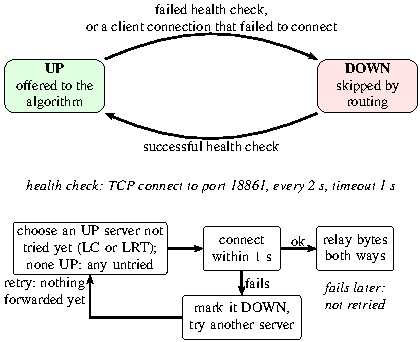
\includegraphics[width=\columnwidth]{figures/health_phase4}
\caption{Failure detection in the LB. Top: status of one server. Bottom: handling of
one client connection; a server that cannot be reached is marked DOWN and the
connection is sent to another server.}
\label{fig:health}
\end{figure}

\begin{figure*}[t]
\centering
\includegraphics[width=0.49\textwidth]{figures/failover-lc-off}\hfill
\includegraphics[width=0.49\textwidth]{figures/failover-lrt-off}\\
\includegraphics[width=0.49\textwidth]{figures/failover-lc}\hfill
\includegraphics[width=0.49\textwidth]{figures/failover-lrt}
\caption{Requests answered per second by each server, and failed requests, while
\texttt{server2} is stopped (first dotted line) and started again (second dotted line).
Left: least connections; right: least response time. Top: without health checks
(Phase 3 LB); bottom: with health checks (Phase 4 LB).}
\label{fig:timeline}
\end{figure*}

\begin{figure}[t]
\centering
\includegraphics[width=\columnwidth]{figures/screenshot_phase4}
\caption{Fault tolerance with least connections: \texttt{docker ps -a} with
\texttt{server2} stopped, and the LB log with \texttt{server2} going DOWN and UP.}
\label{fig:shot-p4}
\end{figure}
